\documentclass[resume]{subfiles}


\begin{document}
\section{U-boot}
\subsection{Compilation}
On configure avec \verb!make uboot-menuconfig! puis on effectue la compilation avec une des deux manières :
\begin{enumerate}
\item \verb!make uboot-rebuild!
\item supprimer les fichiers puis \verb!make!
\end{enumerate}
La configuration de u-boot est stockée dans \verb!.config!
\subsubsection{Amélioration}
Il est possible d'utiliser l'argument \verb!-fstack-protector-all! pour ajouter des vérifications contre les buffer overflows (ou autres attaques sur le stack). Dans ce cas, un canary.\\
Si le canary est écrasé lors de l'éxécution d'un morceau de code. On sais qu'il y a eut un dépassement dans le stack.
\subsection{Démarrage}
Si on appuie sur une touche, on entre en mode u-boot. La commande \verb!booti! permet de lancer l'image linux (\verb!boot! tout court va aussi lancer l'image Linux). Il existe aussi bootz pour charger une image compressée et bootm pour une image fit\\
Avec les commandes présentes dans \verb!boot.cmd!, on indique l'emplacement dans la ram de \verb!Image! et \verb!nanopi-neo-plus.dtb!\\
Lors du démarrage, le Secondary Program Loader (sunxi-spl) va charger le fichier \verb!u-boot.itb!
\subsection{FDT (Flattened Device-Tree)}
Le FDT contient une description hardware du système utilisée par Linux pour sa configuration. le FDT utilise deux fichiers :
\begin{itemize}
\item \verb!.dts! : Device Tree Source (fichier ascii)
\item \verb!.dtb! : Device Tree Blob (fichier binaire)
\end{itemize}
Possibilité de passer de \verb!.dts! à \verb!.dtb! avec la commande \verb!dtc!.\\
U-boot utilise le fichier \\\verb!sun50i-h5-nanopi-neo-plus2.dts! pour configurer Linux sur le NanoPi (information sur le port série, le processeur, etc...).\\
Le FDT est stocké dans le fichier \verb!u-boot.itb!
\subsection{FIT (Flattened Image Tree)}
Nouveau format qui permet d'insérer plusieurs fichiers dans un seul
\begin{figure}[H]
\centering
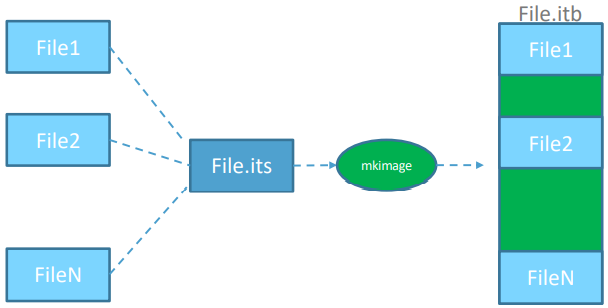
\includegraphics[width=0.75\columnwidth]{img_5.png}
\end{figure}
La commande \verb!mkimage! permet de convertir un fichier \verb!.its! en un fichier \verb!.itb!.\\
Le fichier \verb!u-boot.itb! est construit avec la commande
\begin{center}
\verb!mkimage -f u-boot.its -E u-boot.itb!
\end{center}


\end{document}